% Chapter Template

\chapter{Performance Evaluation} % Main chapter title

\label{Chapter6} % Change X to a consecutive number; for referencing this chapter elsewhere, use \ref{ChapterX}
In this section we present the setup of our two experiment scenarios and we present the positioning results of our experiments in detail.

%----------------------------------------------------------------------------------------
%	SECTION 1
%----------------------------------------------------------------------------------------

\section{Experiment Setup}
We tested our implementation in two complex indoor scenarios with trajectories through numerous of rooms on one floor in a real building of the University of Bern. The first scenario used an area of $715m^2$ and the second scenario $358m^2$. We distributed the UWB anchor nodes over several rooms to cover the area of interest homogenously. The exact position is indicated in the floor plan of figure \ref{fig:anchor_position} for the first scenario and indicated in figure \ref{fig:trajectory5_withAnchors} for the second scenario. In both scenarios the target was hold in the hand of a pedestrian at the starting point of the trajectories, when the experiments started. The pedestrian walked along the given trajectory path, as soon as he passed a predefined checkpoint the current position estimation was registered.\\
\noindent\hspace*{5mm}%
We defined four different trajectories for the first scenario. Each with five to nine checkpoints. Trajectory 1 is indicated in figure \ref{fig:trajectory1}, the other three trajectories can be seen in appendix \ref{AppendixA}. For the second scenario we used a fifth trajectory that covered almost the whole area, it is shown in \ref{fig:trajectory5_withAnchors}.\\
\noindent\hspace*{5mm}%
We repeated the experiments five times, so we analized 145 checking points in scenario 1 and 40 checking points in scenario 2. The localization error was determined by the euclidian distance between the systems position estimation and the real position of the checking point. 



\begin{figure}[th]
\centering
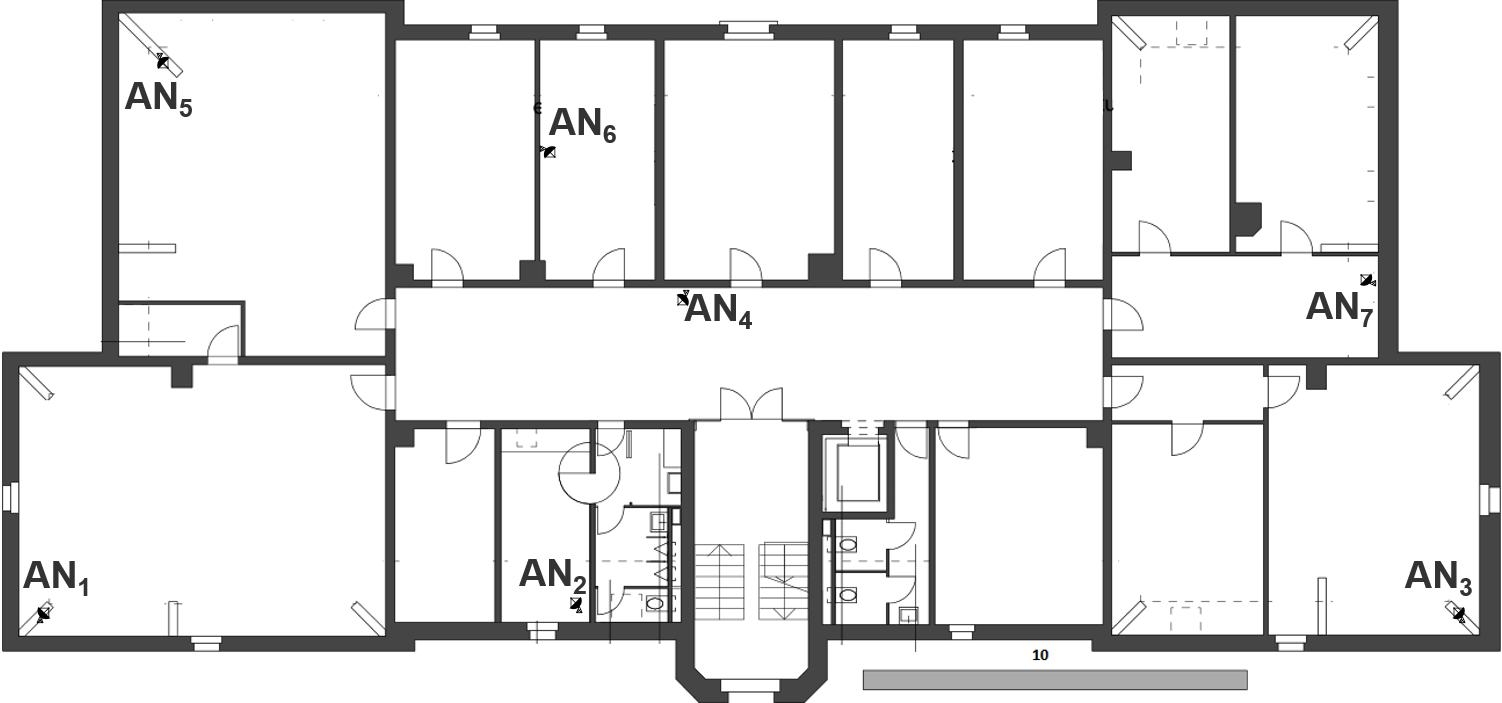
\includegraphics[width=0.8\textwidth]{Figures/anchor_position}
\decoRule
\caption[Anchor node positions]{Distributed anchor nodes on the floor map (with distance reference of 10m).}
\label{fig:anchor_position}
\end{figure}

\begin{figure}[th]
\centering
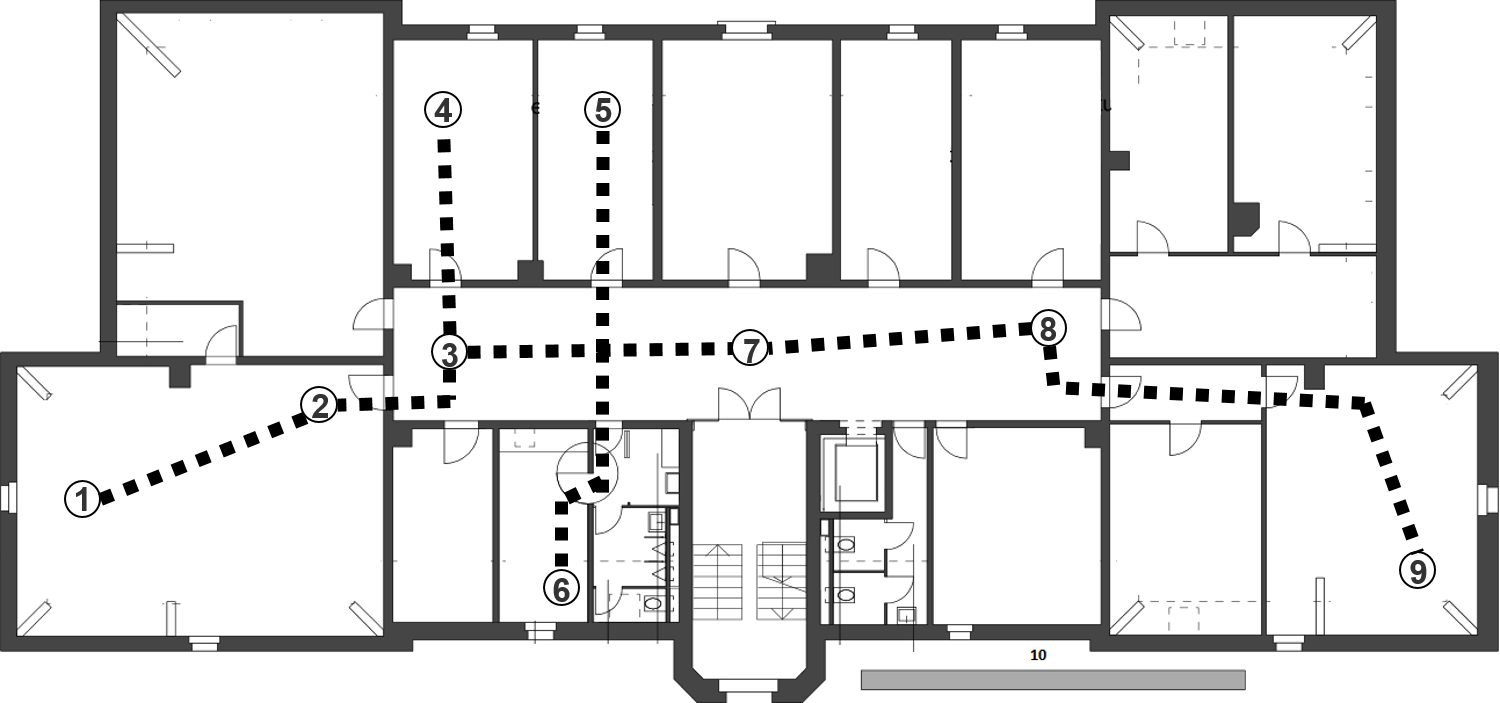
\includegraphics[width=0.8\textwidth]{Figures/trajectory1}
\decoRule
\caption[Trajectory 1]{Trajectory 1 of the four defined trajectories with the position checkpoints.}
\label{fig:trajectory1}
\end{figure}

\begin{figure}[th]
\centering
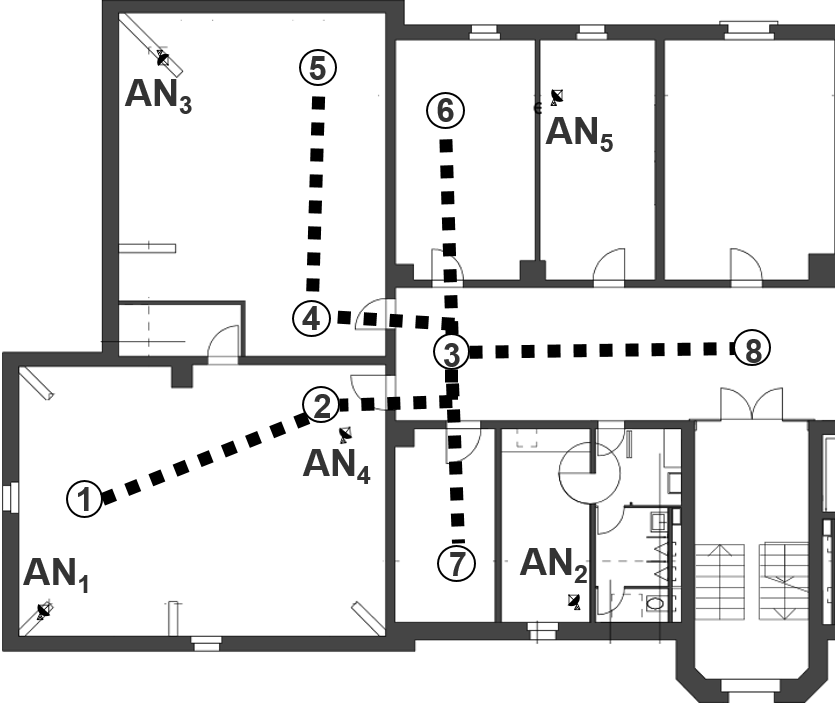
\includegraphics[width=0.5\textwidth]{Figures/trajectory5_withAnchors}
\decoRule
\caption[Trajectory 5]{Trajectory 5 with improved anchor positions.}
\label{fig:trajectory5_withAnchors}
\end{figure}

Zone definition in Testbed.
The zone definition can be seen in figure \ref{fig:zone_definition}, wheras for the smaller scenario (only for trajectory 5) only data in the passed rooms was collected. These were the rooms 1, 2, 3, 5, 6 and 7.  For the wider scenario obviously all indicated rooms were fingerprinted.

\begin{figure}[th]
\centering
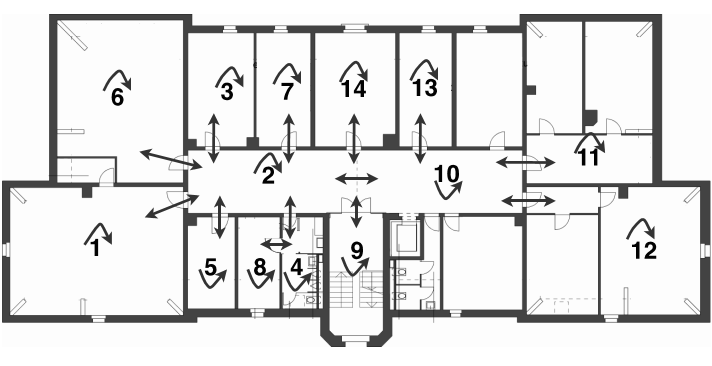
\includegraphics[width=1.0\textwidth]{Figures/zone_definition}
\decoRule
\caption[Zone definition]{Zone definition and transitions between zones}
\label{fig:zone_definition}
\end{figure}


\section{Experiment Results}
In the following the results of our algorithms with a wide distance between anchor nodes are shown. Within this setup we tested trajectory 1 to 4. Each trajectory was tested five times, the results are shown as arithmetic means of these five probes. The anchor node positions for these four tested trajectories are indicated in figure \ref{fig:anchor_position}.

In the first trajectory, the arithmetic mean (hereafter often called average) distance error over all checkpoints was 1.53 meter for $PF_{full}$, 1.47 meter for $PF_{UWBonly}$ and 1.69 meter for Sequiturs commercial system. Looking at figure \ref{fig:trajectory1and2_results}, we see that the errors are often smaller than 1.5 meter, however, there are some checkpoints with very low accuracy. This is also emphasized by comparing the arithmetic mean error to the median error of 1.22m for $PF_{full}$, 0.68m for $PF_{UWBonly}$ and 1.14m for Sequitur, which are significantly lower than the arithmetic means.

The measurements for trajectory two were almost identical, except for $PF_{UWBonly}$, which had no outliers during trajectory 2. The arithmetic mean error for $PF_{full}$ was 2.36m, for $PF_{UWBonly}$ it was 0.55m and for Sequitur 2.26m. Except for $PF_{UWBonly}$, the median errors were again a lot more accurate with 1.07m for $PF_{full}$, 0.49m for $PF_{UWBonly}$ and 1.73m for Sequitur.

\begin{figure}[th]
\centering
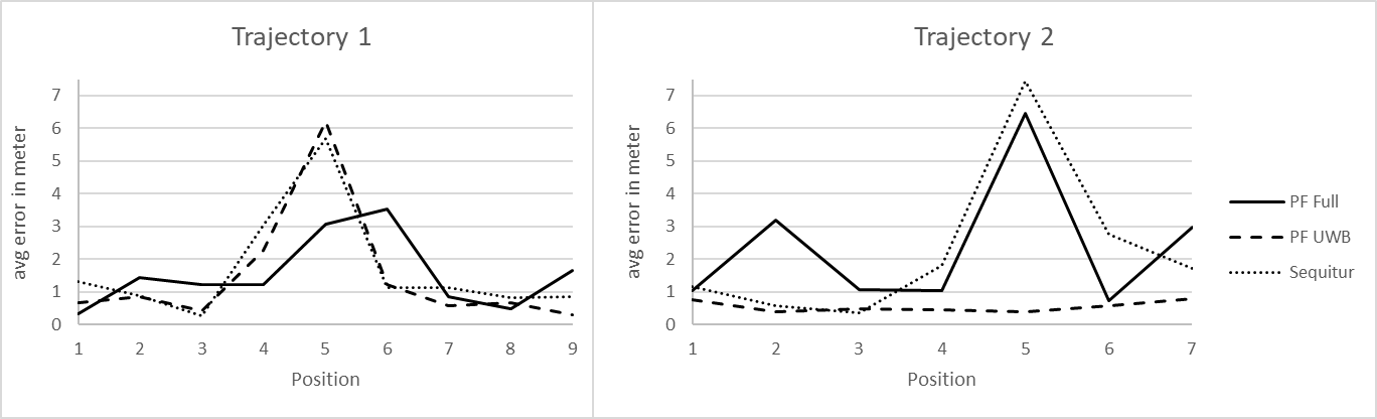
\includegraphics[width=1.0\textwidth]{Figures/trajectory1_2_results}
\decoRule
\caption[Positioning results trajectory 1 and 2]{Graphs of measured distance errors at each checkpoint in trajectory 1, respectively trajectory 2.}
\label{fig:trajectory1and2_results}
\end{figure}

The results for trajectory 3 and 4 were rather similar, however, the peaks observed in figure \ref{fig:trajectory3and4_results} were not as extreme as for the first two trajectories. As above, the average errors in the third trajectory of 1.18m for $PF_{full}$, 0.80m for $PF_{UWBonly}$ and 1.87m for Sequitur were also mentionable higher than the medians of 0.92m, 0.76m and 1.60m.

In the last of these four trajectories no big outliers were stated. Nonetheless the average errors of 1.72m, 1.51m and 1.52m, as well as the median errors 1.26m, 0.68m and 1.24m for $PF_{full}$, $PF_{UWBonly}$ and Sequitur, were still not as accurate as intended.

\begin{figure}[th]
\centering
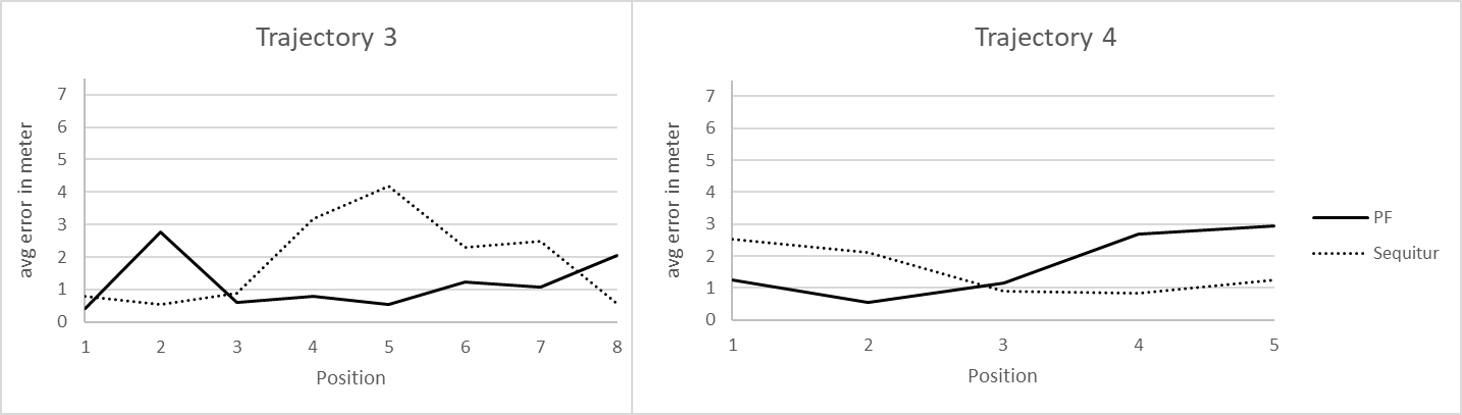
\includegraphics[width=1.0\textwidth]{Figures/trajectory3_4_results}
\decoRule
\caption[Positioning results trajectory 3 and 4]{Graphs of measured distance errors at each checkpoint in trajectory 3, respectively trajectory 4.}
\label{fig:trajectory3and4_results}
\end{figure}

Having a closer look at table \ref{tab:arithmetic_errors}, we see that surprisingly the version of the particle filter only using UWB was the best on every of the trajectories in the low-density anchor node test environment. Moreover, we have seen that there are very big differences between the single checkpoints and even between trajectories. The full variant of the particle filter and the Sequitur system have similar accuracies. For some trajectories one of the algorithms is better, for other trajectories the other performs better. Possible reasons for these volatile results are discussed in the upcoming section \ref{Section2}. 

\begin{table}
\caption{The arithmetic mean of errors in trajectory 1 to 4 (in meter).}
\label{tab:arithmetic_errors}
\centering
\begin{tabular}{l l l l}
\toprule
\textbf{Trajectory} & \textbf{PF Full} & \textbf{PF UWB} & \textbf{Sequitur}\\
\midrule
\textbf{T1} & 1.54 & 1.47 & 1.69\\
\textbf{T2} & 2.36 & 0.55 & 2.26\\
\textbf{T3} & 1.18 & 0.80 & 1.87\\
\textbf{T4} & 1.72 & 1.51 & 1.52\\
\midrule
\textbf{total 1-4}  & \textbf{1.61} & \textbf{1.03} & \textbf{1.79}\\
\bottomrule\\
\end{tabular}
\end{table}

%----------------------------------------------------------------------------------------
%	SECTION 2
%----------------------------------------------------------------------------------------

\section{Comments on low density anchor node test results}
\label{Section2}
The test results in the experiment setup with wide anchor node distances were not as good as intended. To find the reasons for that, we have to carefully have a look at the underlying implementation and the single checkpoint circumstances. We identified two main causes for bad results, they are explained in detail during the next two subsections.
\begin{itemize}
\item Checkpoints outside of AN bounding boxes
\item Failing UWB connection due to too wide distances to ANs
\end{itemize}
These two reasons weren identified in addition to the distractions listed in chapter \ref{Chapter2}. The distractions mentioned for RSSI do also affect UWB signals, especially a cluttered environment will increase - and thus distort - the RTT used for UWB ranging. As in our testing environment servers with iron racks, desks with computer screens as well as a lot of different equipment was present, this effect should not be neglected.

\subsection{Bounding box restrictions}
The AN positions naturally form a bounding box around the environment. The bounding box is the area spanned by straight connections between anchor nodes, as indicated in figure \ref{fig:trajectory1_boundingBox}. Trilateration, also with small distance errors, works well within the bounding box. However even small ranging errors can lead to wrong position estimations outside the bounding box. 
\begin{figure}[th]
\centering
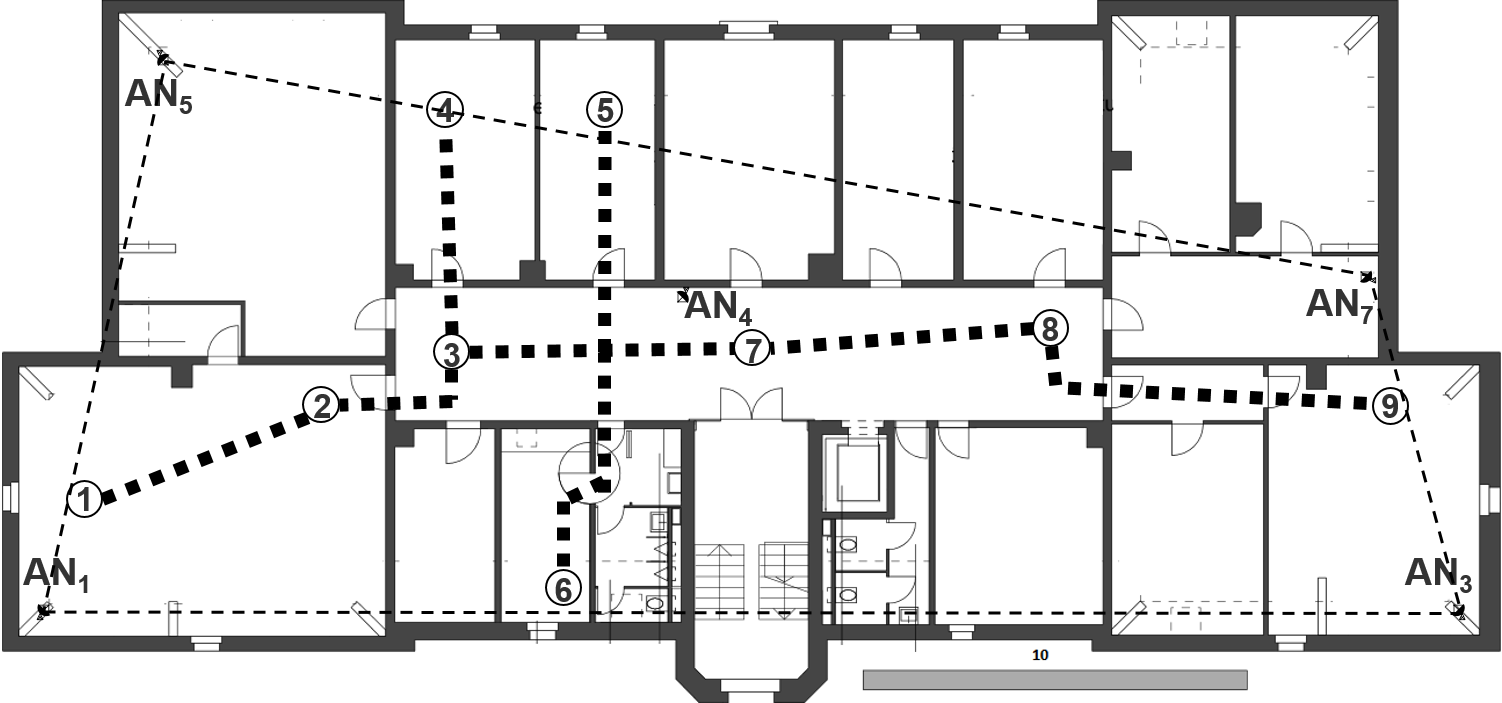
\includegraphics[width=0.8\textwidth]{Figures/trajectory1_boundingBox}
\decoRule
\caption[Bounding box and checkpoints for trajectory 1 ]{Indicated bounding box of the anchor node positions for trajectory 1.}
\label{fig:trajectory1_boundingBox}
\end{figure}
In our experiment especially the results on checkpoint 5 in trajectory 1 and 2 stand out. The average measured errors of 3.09m for $PF_{full}$, 6.23m for $PF_{UWBonly}$ and 5.70m for Sequitur during the first trajectory and 6.46m,  0.38m and 7.45m during the second trajectory are way higher than for other checkpoints. The fact that all of the three algorithms had troubles estimating this position, leads to the conclusion that the experiment setup was the main reason for the big errors at this checkpoint. Moreover, not only lies this point outside the bounding box, but it was also far away from the nearest ANs without a direct line of sight.

\subsection{Failing UWB connections}
All three algorithms depend on a good established UWB connection, as all the ANs ranging estimations are only transmitted via UWB. Especially in the full implementation of the particle filter many UWB meassages are transmitted, because fingerprinting and IMU data are additionally requested and exchanged. For this purpose the radio mode of the UWB devices had to be set to 2, which led to a higher datarate with the cost of lower possible communication distances.\\
For certain checkpoints the distance to the farest anchor nodes were even more than 35m, which was too much for a stable UWB connection with the mentioned configuration. Particularly, the full particle filter had troubles receiving enough usable data, as it produced more overhead than the other algorithms. This led to a high package loss for the full version, such that only one or two range measurements per estimation step were taken into account - instead of the possible five - leading to a higher error. 
\\
\\
During the experiments, we were surprised by the big inaccuracies of all three systems. We intended our system to perform better and in particular the results for Sequitur were surprising, as the UNISET company advertises with centimeter accuracy. This prompted a change in our setup, in order to establish better communication between the nodes with less package loss to enforce more data flowing into the particle filter. 

%----------------------------------------------------------------------------------------
%	SECTION 3
%----------------------------------------------------------------------------------------

\section{Indoor positioning results with high density of anchor nodes}
For trajectory 5 the distances between the anchor nodes were shortened. The exact setup was indicated above in figure \ref{fig:trajectory5_withAnchors}. Equally as before, also trajectory 5 was tested five times, the following results are shown as arithmetic means of these five tests.

As desired the results in this setup were way better than with wider ANs. With an average error of 0.45m for $PF_{full}$, 0.59m for $PF_{UWBonly}$ and 0.48m for Sequitur, this setup outperformed the other trajectories with every algorithm. Even the median errors - with 0.40m, 0.57m and 0.45m -  were not much different, which means that there are no huge differences over the different checkpoints. This can also be seen in figure \ref{fig:trajectory5_results}, where most of the errors are smaller than 0.80m (please note the different axis scale, when comparing with the results for trajectory 1 to 4.

\begin{figure}[th]
\centering
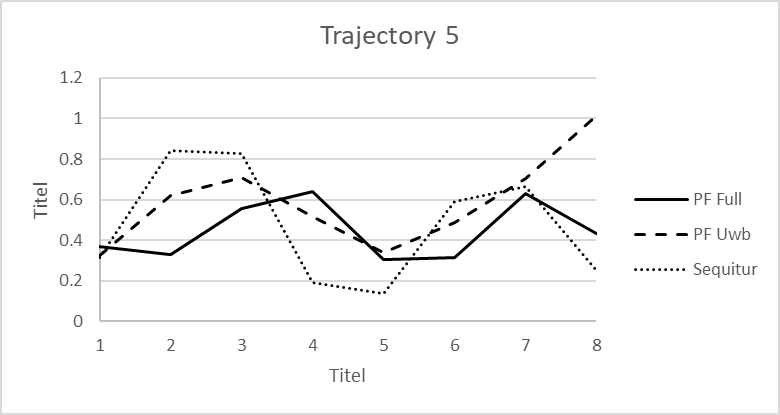
\includegraphics[width=0.8\textwidth]{Figures/trajectory5_results}
\decoRule
\caption[Positioning results trajectory 5]{Graphs of measured distance errors at each checkpoint in trajectory 5.}
\label{fig:trajectory5_results}
\end{figure}

\begin{table}
\caption{The arithmetic mean of errors in trajectory 5 (in meter).}
\label{tab:arithmetic_errors_trajectory5}
\centering
\begin{tabular}{l l l l}
\toprule
\textbf{Trajectory} & \textbf{PF Full} & \textbf{PF UWB} & \textbf{Sequitur}\\
\midrule
\textbf{total 1-4} & 1.61 & 1.03 & 1.79\\
\textbf{T5} & 0.45 & 0.59 & 0.48\\
\midrule
\textbf{difference}  & \textbf{-1.16} & \textbf{-0.44} & \textbf{-1.31}\\
\bottomrule\\
\end{tabular}
\end{table}

In table \ref{tab:arithmetic_errors_trajectory5}, the results of the low density ANs and the high density ANs are compared. The results improved significantly, confirming our suspicion of bad communication affecting the accuracy. With the highest accuracy the full version of the particle filter slightly overcame the Sequitur commercial system. The particle filter only taking UWB ranging into account was more accurate too, however, the improvement was not as big as for the two other algorithms.

%----------------------------------------------------------------------------------------
%	SECTION 4
%----------------------------------------------------------------------------------------

\section{Comments on high density anchor node test results}
\label{Section4}
With the more dense spread of the ANs, the estimations improved a lot. Having a look at our two assumptions from section \ref{Section2}, we can state the following:

\begin{itemize}
\item Checkpoints outside of AN bounding boxes had quite good accuracy, adding doubts to this explanation.
\item The communication was better, what improved the accuracy a lot and confirmed our assumption.
\end{itemize}

\subsection{Bounding box restrictions}
In the new setup we purposely added checkpoints at the edge or outside the bounding box, as seen in figure \ref{fig:trajectory5_boundingBox}. Especially checkpoint 5 and 8 are not lying within the bounding box, however they still had a quite good accuracy. For checkpoint 5 the average estimation errors were 0.30m, 	0.34m, and 0.14m, for checkpoint 8 the errors were 0.43m,	1.01m and 0.25m for $PF_{full}$, $PF_{UWBonly}$ and Sequitur. It made no difference for the tag being outside the bounding box or not. We conclude that with good ranging data it is not very important to stay within the bounding box, however, wrong ranging data leads to bigger errors outside the bounding box.

\begin{figure}[th]
\centering
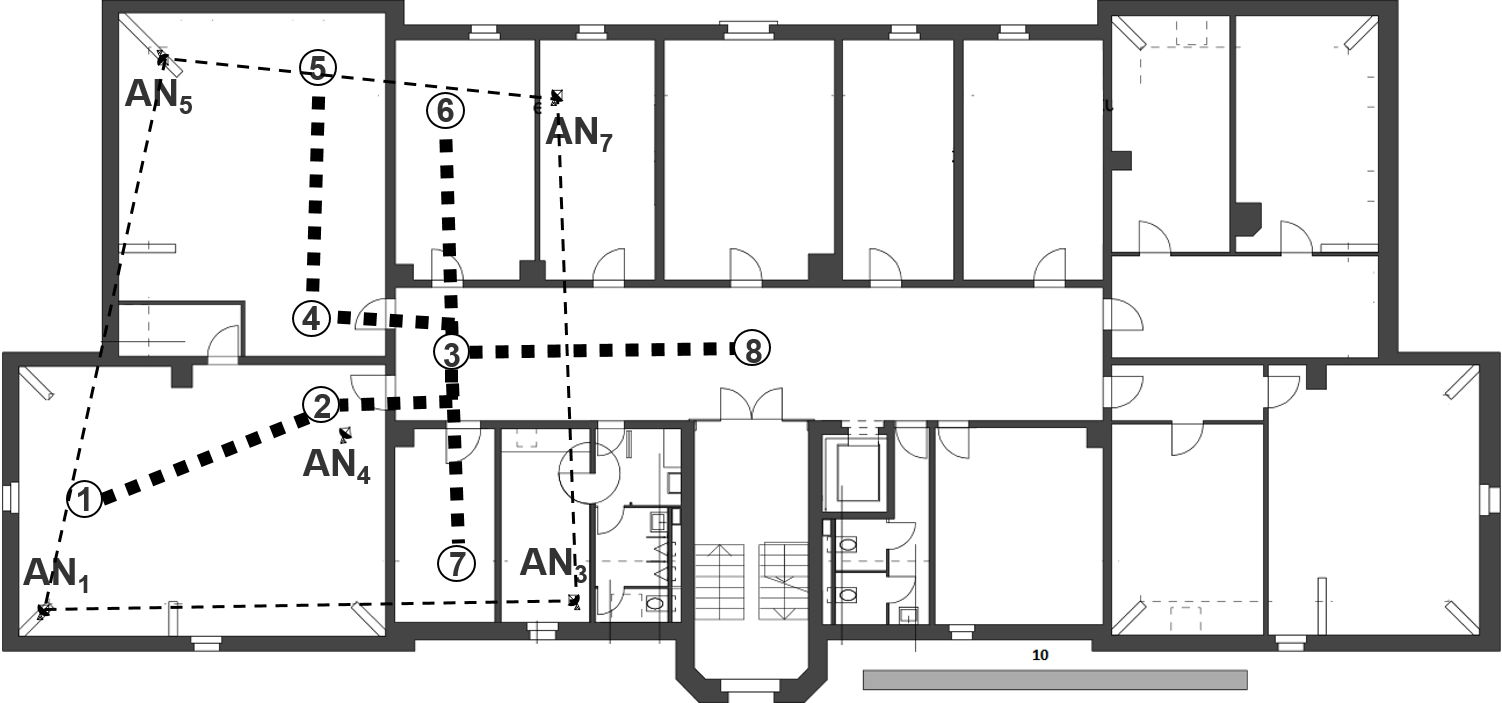
\includegraphics[width=0.8\textwidth]{Figures/trajectory5_boundingBox}
\decoRule
\caption[Trajectory 5 with bounding box]{Indicated bounding box of the anchor node positions for trajectory 5.}
\label{fig:trajectory5_boundingBox}
\end{figure}

\subsection{Failing UWB connections}
A bigger influence on the estimation error has the UWB connection. With a better established connection - in our case with nearer ANs - more UWB messages arrived at the receiver. In each estimation step, more data was fed into the positioning algorithms what caused obviously a more precise performance. For the full version of the particle filter the communication is one of the key performance values, because the data is requested serially. This only allowes a limited amount of retransmitting and the communication timeouts have to be kept short. The resulting increased package loss affects the data quality,  such that some evaluating steps were skipped. Obviously the lack of data led to bad results, as the particle filter improves its estimation by fusing many different measurements, what is not possible when a part of the data is not present. 
